\chapter{Appendix A}
\section{VHDL module specifications}

\subsection{Adder}

\begin{figure}[h]
    \centering
    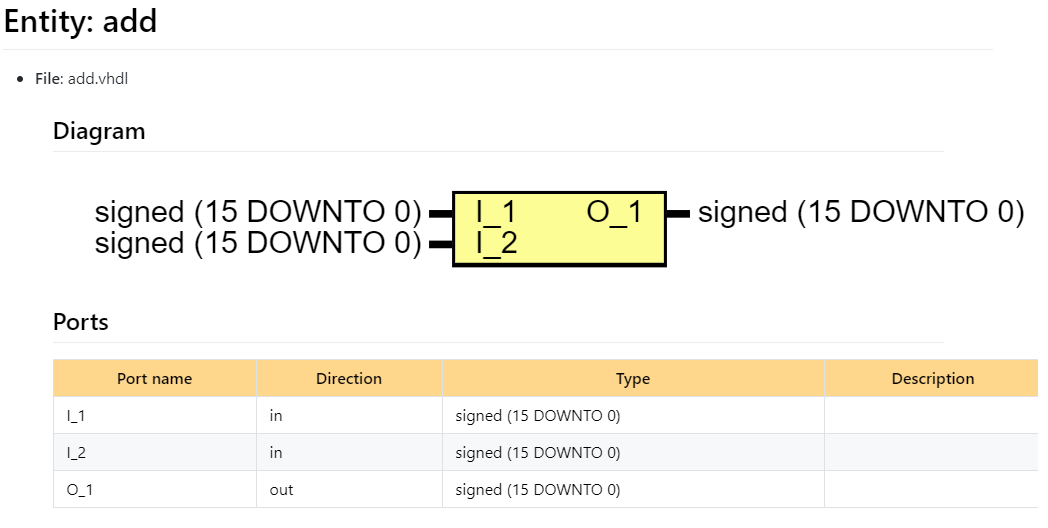
\includegraphics[width=0.9\textwidth]{adder_specs.png}
    \caption{Adder specifications}
    \label{fig:adder_specs}
\end{figure}

\subsection{Multiplier}

\begin{figure}[h]
    \centering
    \includegraphics[width=0.9\textwidth]{Mul_specs.png}
    \caption{Mul specifications}
    \label{fig:mul_specs}
\end{figure}

\subsection{D-FlipFlop}

The D-FlipFlop supports both synchronous and asynchronous resets.

\begin{figure}[h]
    \centering
    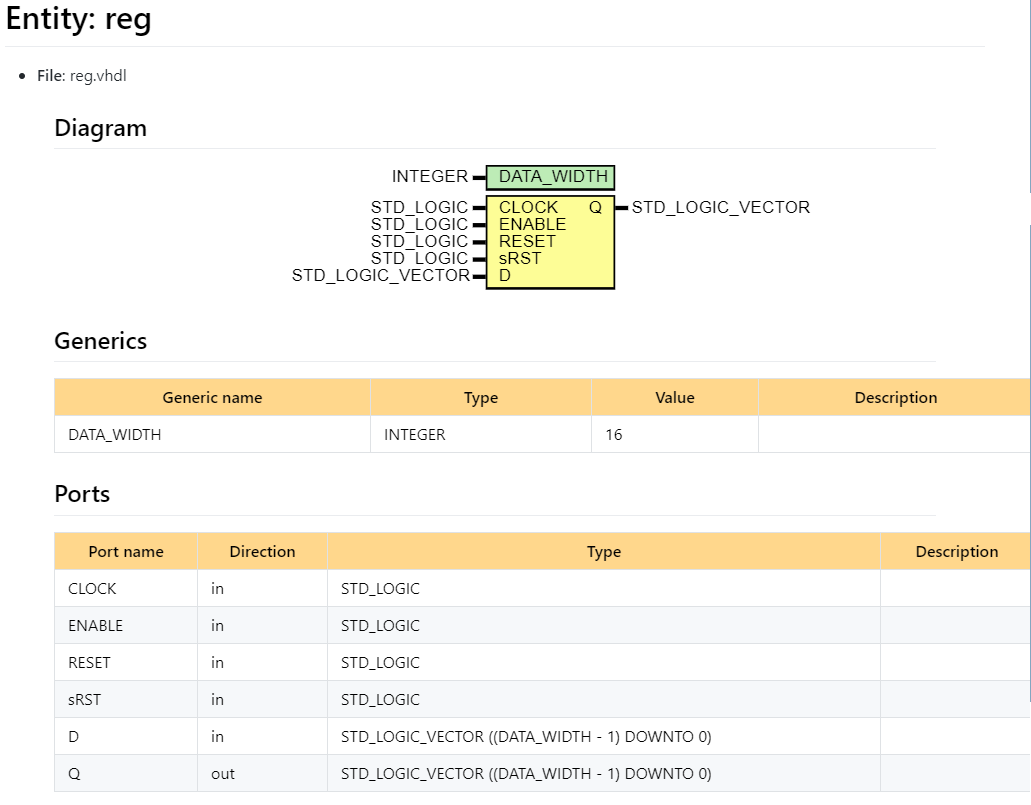
\includegraphics[width=0.6\textwidth]{reg_specs.png}
    \caption{FlipFlop specifications}
    \label{fig:reg_specs}
\end{figure}

\subsection{Peak Detector}

\begin{figure}[h]
    \centering
    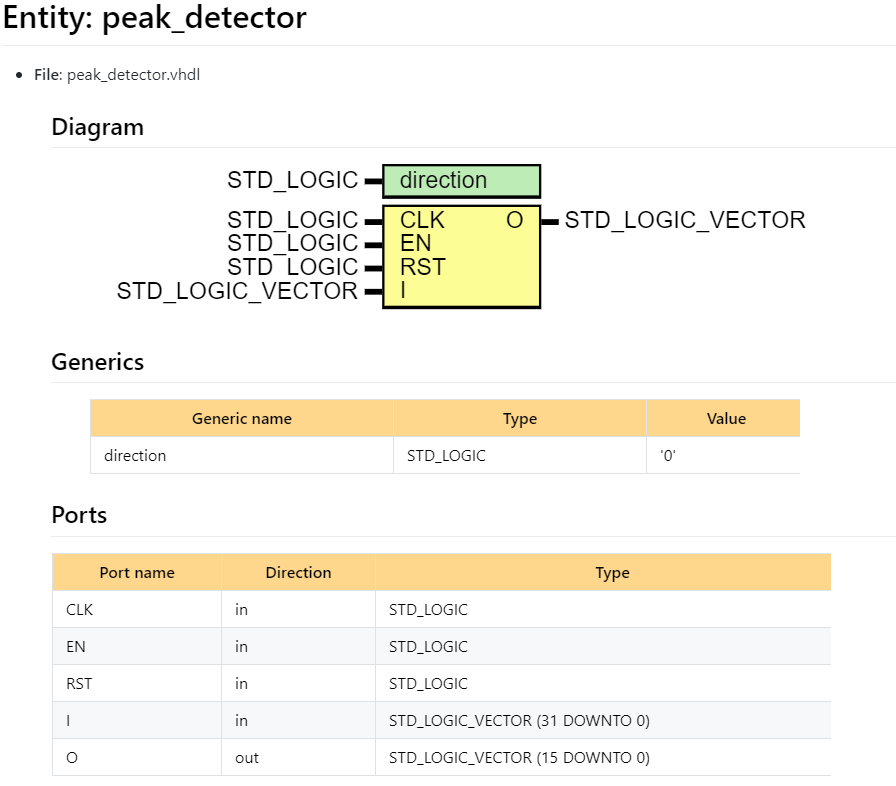
\includegraphics[width=0.6\textwidth]{peak_specs.png}
    \caption{Peak Detector specifications}
    \label{fig:peak_specs}
\end{figure}



